
% Inbuilt themes in beamer
\documentclass[aspectratio=169]{beamer}
\usepackage{graphicx}
\usepackage{mathrsfs}
% Theme choice:
\usetheme{CambridgeUS}

% Title page details: 
\title{Econometrics Discussion Section 2} 
\author{John Green}
\date{Spring 2024}


\begin{document}

% Title page
\begin{frame}
    \titlepage 
\end{frame}

% Outline frame
\begin{frame}{Linear regression}
    We now want to move on to examining how to understand the relationship between two variables.
    \begin{itemize}
        \item Linear regression model
        \item Necessary assumptions
        \item $R^2$, SER, F-test
        \item Distinguish \textit{prediction} from \textit{causation}
    \end{itemize}
\end{frame}

\begin{frame}{Minimizing error with one variable}
    \begin{itemize}
        \item Suppose we have data $X_1, X_2, X_3, \ldots, X_n = \{ X_i \}_{i \leq n} $
        \item What is the best guess for the value of an arbitrary $X_j$?
        \begin{itemize}
            \item The best fit will be the mean, $ E[X] $
        \end{itemize}
        \item But wait: which error are we minimizing?
    \end{itemize}
\end{frame}

\begin{frame}{Minimizing error with one variable}
    \begin{itemize}
        \item Suppose we have data $X_1, X_2, X_3, \ldots, X_n = \{ X_i \}_{i \leq n} $
        \item What is the best guess for the value of an arbitrary $X_j$?
        \begin{itemize}
            \item The best guess is going to be the mean, $ E[X] $
            \item This is intuitively embedded in the language we use: the ``expectation'' of $X$
        \end{itemize}
        \item But wait: which error are we minimizing?
    \end{itemize}
\end{frame}

\begin{frame}{Minimizing error with one variable}
    \begin{itemize}
        \item Suppose we have data $X_1, X_2, X_3, \ldots, X_n = \{ X_i \}_{i \leq n} $
        \item What is the best guess for the value of an arbitrary $X_j$?
        \begin{itemize}
            \item The best guess is going to be the mean, $ E[X] $
            \item This is intuitively embedded in the language we use: the ``expectation'' of $X$
        \end{itemize}
        \item But wait: which error are we minimizing?
        \begin{itemize}
            \item \textit{Mean squared error}
        \end{itemize}
    \end{itemize}
\end{frame}

\begin{frame}{Minimizing mean squared error}
   Our problem:
   $$
    \underbrace{\text{arg min}}_{f} \mathbb{E}\left[\frac{1}{2}(X - f)^2\right]
   $$
   How do we find the $f$ that minimizes this?
\end{frame}

\begin{frame}{Minimizing mean squared error}
    Our problem:
    $$
    \underbrace{\text{arg min}}_{f} \mathbb{E}\left[\frac{1}{2}(X - f)^2\right]
    $$
    How do we find the $f$ that minimizes this? 

    \vspace{2mm}

    \textbf{Set the derivative to 0:}

    $$
    \mathbb{E}[(X-f)] = 0 \iff f = \mathbb{E}[X]
    $$
 \end{frame}

\begin{frame}{Minimizing error with two variables}
    \begin{itemize}
        \item Now what if we have data on two variables:
        $$
        (X_1, Y_1), (X_2, Y_2), \ldots, (X_n, Y_n) = \{ (X_i, Y_i) \}_{i \leq n}
        $$
        \item We want to understand their relationship! 
        \item What is our best guess for an arbitrary $Y_j$, given $X_j$?
        \begin{itemize}
            \item $X$ is age and $Y$ is income; if I tell you that someone is 20 years old, what is your best guess for their income?
            \item This will be the \textit{conditional expectation}: $E[Y|X=20]$
        \end{itemize}
    \end{itemize}
\end{frame}

\begin{frame}{Minimizing error with two variables}
    \begin{itemize}
        \item What is our best guess for an arbitrary $Y_j$, given $X_j$?
        \begin{itemize}
            \item $X$ is age and $Y$ is income; if I tell you that someone is 20 years old, what is your best guess for their income?
            \item This will be the \textit{conditional expectation}: $E[Y|X=20]$
        \end{itemize}        
        \item Let's assume a \textit{linear} relationship:
        $$
        Y_i = \beta_0 + \beta_1 X_i
        $$
        \item Then our problem is to draw a line through the 2D data which minimizes the errors
        \begin{itemize}
            \item $\beta_0$ is the intercept, $\beta_1$ is the slope
        \end{itemize}
    \end{itemize}
\end{frame}

\begin{frame}
    \centering
    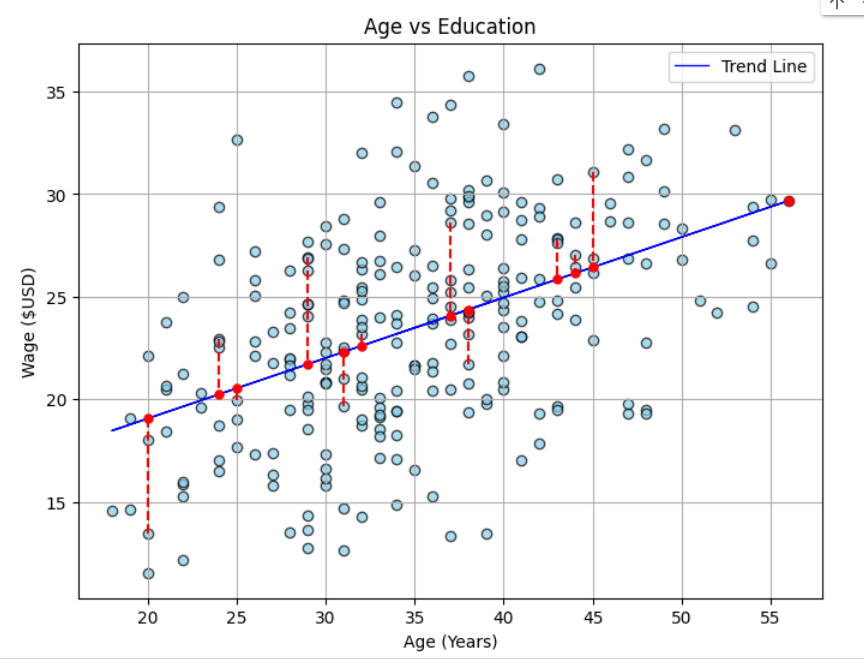
\includegraphics[width = .6\textwidth,keepaspectratio]{./figs/age_ed.png}
\end{frame}

\begin{frame}{Ordinary least squares}
    \begin{itemize}
        \item The line which minimizes the errors is the \textit{ordinary least squares} regression line
        \item Found by solving 
        $$
        \min_{\beta_0, \beta_1} \sum_{i=1}^n (Y_i - (\beta_0 - \beta_1 X_i))^2
        $$
        just like we did before (derived in lecture notes and book)
        \item In practice, we only have a \textbf{sample}, and so we have to estimate these two parameters:
        \begin{itemize}
            \item Add an error term: $Y_i = \beta_0 + \beta_1 X_i + \epsilon_i$
            \item We will denote these estimates as $\hat{\beta}_0$ (intercept) and $\hat{\beta}_1$ (slope)
        \end{itemize}
    \end{itemize}
\end{frame}

\begin{frame}{Assumptions}
    \begin{itemize}
        \item What assumption have we made so far?
    \end{itemize}
\end{frame}

\begin{frame}{Assumptions}
    \begin{itemize}
        \item What assumption have we made so far?
        \begin{itemize}
            \item Specified a \textbf{linear} relationship between $X$ and $Y$
            \item This is not a small assumption!
        \end{itemize}
        \item What if we want to think about $X$ as having a causal effect on $Y$?
        \begin{itemize}
            \item eg if we were to hold all other factors constant (as in a controlled and randomized experiment) what do we expect an extra year of education to do to income?
        \end{itemize}
    \end{itemize}
\end{frame}

\begin{frame}{Assumptions}
    For $\beta_1$ to have a \textit{causal} interpretation, several assumptions are necessary:
    \begin{enumerate}
        \item $E[\epsilon | X=x] = 0$ 
        \begin{itemize}
            \item So that $\hat{\beta_1}$ is unbiased estimator
        \end{itemize}
        \item $\{ (X_i, Y_i) \}_{i \leq n}$ are i.i.d. 
        \begin{itemize}
            \item Will give us sampling distributions for coefficient estimates
        \end{itemize}
        \item Large outliers are rare 
        \begin{itemize}
            \item OLS is sensitive to outliers, and our estimate $\hat{\beta}$ might be meaningless otherwise
        \end{itemize}
    \end{enumerate}
\end{frame}

\begin{frame}{Exogeneity}
    \begin{itemize}
        \item $E[\epsilon | X=x] = 0$ implies that $X$ is \textit{exogeneous}
        \begin{itemize}
            \item Uncorrelated with the error term
        \end{itemize}
        \item When might this fail?
    \end{itemize}
\end{frame}

\begin{frame}{Omitted variable bias}
    \begin{itemize}
        \item $E[\epsilon | X=x] = 0$ implies that $X$ is \textit{exogeneous}
        \begin{itemize}
            \item Uncorrelated with the error term
        \end{itemize}
        \item When might this fail?
        \item If there is an omitted variable that is correlated with $X$ and $Y$, then $X$ is not exogeneous
        \item Suppose we regress years of education on wages:
        $$
            W_i = \beta_0 + \beta_1 E_i + \epsilon_i
        $$
        \item What might an omitted variable be?
    \end{itemize}
\end{frame}

\begin{frame}{Omitted variable bias}
    \begin{itemize}
        \item Suppose we regress years of education on wages:
        $$
            W_i = \beta_0 + \beta_1 E_i + \epsilon_i
        $$
        \item What might an omitted variable be?
        \item Suppose parental income is correlated with both years of education and wages, so the true model is:
        $$
            W_i = \beta_0 + \beta_1 E_i + Z_i + u_i
        $$
        \item So when we estimate the first model, $\epsilon_i = Z_i + u_i $ and exogeneity will fail
    \end{itemize}
\end{frame}

\begin{frame}{Intuition behind exogeneity}
    \begin{itemize}
        \item $\epsilon_i$ contains all of the things that influence $Y_i$ that are not explicitly included in our model
        \item So, $E[\epsilon | X=x] = 0$ means that none of those factors are correlated with $X$
        \item $\epsilon_i$ will \textbf{always} contain extra terms we have not included, since there are always unobserved variables
        \item The problem only emerges when such variables are correlated with the included $X$
    \end{itemize}
\end{frame}

\begin{frame}{Regression output}
    \begin{itemize}
        \item $R^2$ measures the variance in $Y$ that is explained by $X$
        \begin{itemize}
            \item $R^2 = \frac{ESS}{TSS}$
        \end{itemize}
        \item Standard error of regression (SER): spread of the residual $\epsilon$
        \item Root mean squared error (RMSE): similar, just calculated with $n$ instead of $n-2$ in the denominator
    \end{itemize}
\end{frame}

\begin{frame}{Sampling distribution of $\hat{\beta}$}
    \begin{itemize}
        \item Just like $\bar{Y}$, $\hat{\beta}$ is a random variable and has a sampling distribution! (Why?)
        \item So, if we want to be able to say something about the relationship between an $X$ and a $Y$ using $\hat{\beta}$, we need to know something about its distribution
        \begin{itemize}
            \item Will allow us to test hypotheses, eg that $\beta_1 = 0$
            \item Will let us construct confidence intervals and indicate uncertainty
        \end{itemize}
        \item Extra assumption on top of the OLS assumptions: that the relationship between $X$ and $Y$ is linear (how might we relax this?)
    \end{itemize}
\end{frame}

\begin{frame}{Hypothesis testing for $\hat{\beta}$}
    \begin{itemize}
        \item Will work in a very similar way to the hypothesis testing we've done for the sample mean
        \begin{itemize}
            \item Variance of $\hat{\beta}$ is decreasing in the sample size and in the variance of $X$
        \end{itemize}
        \item We will construct a t-statistic, $t=\frac{\hat{\beta}-\beta}{SE(\hat{\beta})}$
        \item So we can test if $\beta=0$ (ie if $X$ has no relationship with $Y$), or if $\beta<0$ (ie $X$ has a negative relationship with $Y$)
        \item Can CIs as well
    \end{itemize}
\end{frame}

\begin{frame}{Binary regression}
    \begin{itemize}
        \item Sometimes we have a binary regressor: for example, participation in some program
        \begin{itemize}
            \item Effect of taking a drug
        \end{itemize}
        \item OLS works in the same way but interpretation is a little different:
        \begin{itemize}
            \item $Y_i = \beta_0 + \beta_1 D_i + \epsilon_i$
            \item $\beta_0$ is mean with no treatment
            \item $\beta_0 + \beta_1$ is the mean with treatment
            \item So $\beta_1$ is the average treatment effect
        \end{itemize}
    \end{itemize}
\end{frame}

\begin{frame}{Heteroskedasticity}
    \begin{itemize}
        \item Homoskedasticity: $\epsilon$ has constant variance (doesn't depend on X)
        \item If we assume Homoskedasticity, we can say some stronger things about the OLS
        \begin{itemize}
            \item Gauss-Markov theorem: OLS is the best linear unbiased estimator ie has smallest variance
            \item Simpler formula for the variance of $\hat{\beta}$
        \end{itemize}
        \item What if we assume Homoskedasticity but it's not true?
        \begin{itemize}
            \item SE will be too small (probably) meaning that we are \textit{overconfident} in our inference
        \end{itemize}
        \item If we assume normal errors, we can say some even stronger things
        \item Make strong assumptions, get strong results! These are usually difficult to justify.
    \end{itemize}
\end{frame}


\begin{frame}{Consistency and bias}
    \begin{itemize}
        \item There are many features we would like our estimators to have: being \textit{consistent} and \textit{unbiased} are (usually) two of them
        \item Let's say we have an estimator $\hat{\theta}(x_i)$ for some statistic $\theta$
        \begin{itemize}
            \item $\bar{x}$ is estimator for $\mu_x$, $\hat{\beta}^{OLS}$ is estimator for $\beta$
            \item In other words, we look at some data $x_i$, use it to come up with a ``best guess'' for the $\theta$
        \end{itemize}
        \item Consistent: as our sample size grows, the estimator converges to the true value of the parameter
        \begin{itemize}
            \item $\hat{\theta}(x_i) \xrightarrow{p} \theta$
        \end{itemize}
        \item Unbiased: in expectation, our estimator is equal to the true value of the parameter
        \begin{itemize}
            \item $\mathbb{E}[\hat{\theta}(x_i) - \theta] = 0 $
        \end{itemize}
    \end{itemize}
\end{frame}

\begin{frame}{Showing consistency and unbiasedness}
    \begin{itemize}
        \item Bias is usually straightforward to show: take the expectation of the estimator, try to show it is equal to the object of interest
        \item Consistency is (sometimes) trickier
        \item 3 main tools to take advantage of:
        \begin{itemize}
            \item Law of large numbers: as $n \to \infty$, $\bar{x} \xrightarrow{p} \mu_x$
            \item Central limit theorem: as $n \to \infty$, $\sqrt{n}(\bar{x} - \mu_x) \xrightarrow{d} N(0, \sigma^2)$ eg $\bar{x} \xrightarrow{d} N(\mu_x, \dfrac{\sigma^2}{n})$
            \item Continuous mapping theorem: if $X_n \xrightarrow{p} X$, $Y_n \xrightarrow{p} Y$, then for continuous functions $g$, $g(X_n, Y_n) \xrightarrow{p} g(X,Y)$
        \end{itemize}
        \item Nothing complicated: just take things piece by piece and ask yourself what happens when n gets big
    \end{itemize}
\end{frame}

\begin{frame}{Sample mean}
    \begin{itemize}
        \item Random variable $X_i \sim F$, let $\mathbb{E} [X_i] = \mu_x$ and $\text{Var}(X_i) = \sigma^2$
        \item Sample mean: $\bar{x} = \frac{1}{n} \sum_{i=1}^n x_i$
        \item Is it biased?
    \end{itemize}
\end{frame}

\begin{frame}{Sample mean}
    \begin{itemize}
        \item Random variable $X_i \sim F$, let $\mathbb{E} [X_i] = \mu_x$ and $\text{Var}(X_i) = \sigma^2$
        \item Sample mean: $\bar{x} = \frac{1}{n} \sum_{i=1}^n x_i$
        \item Is it biased?
        $$
        \mathbb{E}[\bar{x}] = \mathbb{E}\left[\frac{1}{n} \sum_{i=1}^n x_i\right] = \frac{1}{n} \sum_{i=1}^n \mathbb{E}[x_i] = \frac{1}{n} n \mu_x = \mu_x
        $$
        Unbiased!
        \item Is it consistent?
    \end{itemize}
\end{frame}

\begin{frame}{Sample mean}
    \begin{itemize}
        \item Random variable $X_i \sim F$, let $\mathbb{E} [X_i] = \mu_x$ and $\text{Var}(X_i) = \sigma^2$
        \item Sample mean: $\bar{x} = \frac{1}{n} \sum_{i=1}^n x_i$
        \item Is it biased?
        $$
        \mathbb{E}[\bar{x}] = \mathbb{E}\left[\frac{1}{n} \sum_{i=1}^n x_i\right] = \frac{1}{n} \sum_{i=1}^n \mathbb{E}[x_i] = \frac{1}{n} n \mu_x = \mu_x
        $$
        Unbiased!
        \item Is it consistent?
        \begin{itemize}
            \item Of course -- this is exactly what the LLN tells us
            $$
                \bar{x} \xrightarrow{p} \mu_x
            $$
        \end{itemize}
    \end{itemize}
\end{frame}

\begin{frame}{Consistency and bias}
    \begin{itemize}
        \item Does bias $\rightarrow$ consistency? \textbf{No!}
    \end{itemize}
\end{frame}

\begin{frame}{Consistency and bias}
    \begin{itemize}
        \item Does bias $\rightarrow$ consistency? \textbf{No!}
        \item Does consistency $\rightarrow$ bias?
    \end{itemize}
\end{frame}

\begin{frame}{Consistency and bias}
    \begin{itemize}
        \item Does bias $\rightarrow$ consistency? \textbf{No!}
        \item Does consistency $\rightarrow$ bias? \textbf{Not true either.}
    \end{itemize}
\end{frame}


\begin{frame}[shrink]
    \frametitle{Consistent but biased}
    \begin{figure}[htbp]
        \centering
        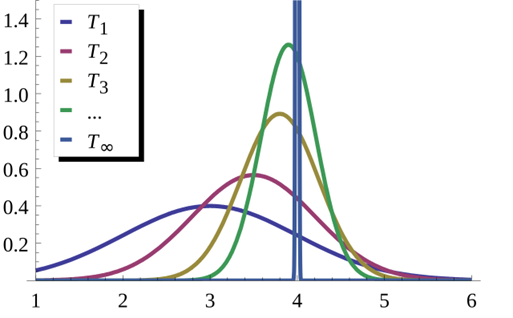
\includegraphics[width=0.75\textwidth]{./consistency.png}
    \end{figure}
\end{frame}

\begin{frame}{Consistent but biased}
    \begin{itemize}
        \item Remember that our estimator for the sample mean is:
        $$
            \hat{\sigma}^2 = \frac{1}{n-1} \sum_{i=1}^n (x_i - \bar{x})^2
        $$
        \item This is because the naive estimator is biased:
        \begin{equation*}
            \begin{split}
                \hat{\sigma}_{naive}^2 & = \frac{1}{n} \sum_{i=1}^n (x_i - \bar{x})^2 \\
                \rightarrow & \\
                \mathbb{E} [\hat{\sigma}_{naive}^2] & = \dfrac{n-1}{n} \sigma^2
            \end{split}
        \end{equation*}
        \item So there is a bias term of $\dfrac{n-1}{n}$
        \item But is this estimator consistent?
    \end{itemize}
\end{frame}

\begin{frame}{Consistent but biased}
    \begin{itemize}
        \item The naive estimator is biased:
        \begin{equation*}
            \begin{split}
                \hat{\sigma}_{naive}^2 & = \frac{1}{n} \sum_{i=1}^n (x_i - \bar{x})^2 \\
                \rightarrow & \\
                \mathbb{E} [\hat{\sigma}_{naive}^2] & = \dfrac{n-1}{n} \sigma^2
            \end{split}
        \end{equation*}
        \item So there is a bias term of $\dfrac{n-1}{n}$
        \item But is this estimator consistent?
        \begin{itemize}
            \item Yes, since $\text{lim}_{n \to \infty} \dfrac{n-1}{n} = 0$
        \end{itemize}
    \end{itemize}
\end{frame}

\begin{frame}{Unbiased but not consistent}
    \begin{itemize}
        \item What if we use an extremely naive estimator for $\mu_x$: $X_1$
        \begin{itemize}
            \item Take a sample, take the first value, that's our estimator
        \end{itemize}
        \item Is this biased?
    \end{itemize}
\end{frame}

\begin{frame}{Unbiased but not consistent}
    \begin{itemize}
        \item What if we use an extremely naive estimator for $\mu_x$: $X_1$
        \begin{itemize}
            \item Take a sample, take the first value, that's our estimator
        \end{itemize}
        \item Is this biased?
        \begin{itemize}
            \item No: $\mathbb{E} [ X_1] = \mu_x $
        \end{itemize}
        \item Is it consistent?
    \end{itemize}
\end{frame}

\begin{frame}{Unbiased but not consistent}
    \begin{itemize}
        \item What if we use an extremely naive estimator for $\mu_x$: $X_1$
        \begin{itemize}
            \item Take a sample, take the first value, that's our estimator
        \end{itemize}
        \item Is this biased?
        \begin{itemize}
            \item \textbf{No}: $\mathbb{E} [ X_1] = \mu_x $
        \end{itemize}
        \item Is it consistent?
        \begin{itemize}
            \item \textbf{No}: $X_1 \sim F$ and does not depend on $n$; so as $n \to \infty$, $X_1$ does not converge to $\mu_x$
        \end{itemize}
    \end{itemize}
\end{frame}

\begin{frame}{Bias and consistency}
    \begin{itemize}
        \item To sum up: in general, we like unbiased and consistent estimators
        \item Take expectation to check for bias; use CLT + CMT for consistency
        \item Bias != consistency, and consistency != bias
        \item Our favorite estimators, eg $\frac{1}{n} \sum_i x_i $ and $\hat{\beta}^{OLS}$, are both consistent and unbiased
    \end{itemize}
\end{frame}

\begin{frame}{Prediction}
    \begin{itemize}
        \item Oftentimes, we are just concerned with predicting a Y-variable:
        $$
            \hat{Y}_i = \hat{\beta}_0 + \hat{\beta}_1 X_i
        $$
        \item Will always have some error in our prediction; but important to think about where it comes from
        \item In general (and in particular with the OLS model) we have at least two sources of error:
        \begin{itemize}
            \item The intrinsic error in predicting an uncertain outcome (``oracle'' error; $V_1$ in slides); $\mathbb{E}[u_i^2]$
            \item Additional error introduced because we are estimating our model with a random sample (``estimation'' error; $V_2$ in slides); $\mathbb{E}\left[\left(\left(\hat{\beta}_0-\beta_0\right)+x_0\left(\hat{\beta}_1-\beta_1\right)\right)^2 \mid X=x_0\right]$
        \end{itemize}
    \end{itemize}
\end{frame}

\begin{frame}{Prediction}
    \begin{itemize}
        \item We want to account for both of these when we make a prediction (see example)
        \item If we only account for sampling error, we will be overconfident in our prediction 
        \item So, what to do if we want to make good predictions?
        \item OLS estimator will not be best for out of sample predictions
        \item Later on, will explore the ``bias-variance'' tradeoff: we may intentionally introduce some bias into our model in order to reduce the variance due to the estimated coefficients, thus getting the error in our model closer to the oracle prediction
    \end{itemize}
\end{frame}

\end{document}